% article example for classicthesis.sty
\documentclass[10pt,a4paper]{article} % KOMA-Script article scrartcl
\usepackage{lipsum}
\usepackage{url}
\usepackage[nochapters]{../classicthesis} % nochapters
\usepackage{graphicx}
\graphicspath{ {img/} }
\usepackage{booktabs}
\usepackage{float}









usepackage{hyperref}

\begin{document}
    \pagestyle{plain}
    \title{\rmfamily\normalfont\spacedallcaps{Mission: Chuckhole}}
    \author{\spacedlowsmallcaps{Marwan ElMezni, Michael Moosbauer}}
    \date{} % no date
    
    \maketitle
    
%    \begin{abstract}
        %Maybe we won't need an abstract
 %   \end{abstract}
 
\newpage
    \tableofcontents
\newpage    
    \section{Motivation and problem statement}



Even though municipalities try to maintain and repair roads, many segments still contain chuckholes that vehicle owners prefer to avoid to drive or to bike on because they would so likely damage their vehicles and slow or interrupt the traffic.

This was the background motivation to develop a mobile application, in a biking context, that helps users to avoid damaged sections of roads or to detect and localize chuckholes.

 
 
 
 
    \section{Recommended Setup}
	%photo of bike, smartphone fix, ...    
	\begin{itemize} 
	\item Bike: Drössiger 650B full suspension.
	\item Smartphone (Samsung Galaxy S4 Active).
	\item Fix spot of the mobile phone: on the handlebar.
	
	
	\end{itemize}
	% send me a picture of your bike with the fix and the phone


    \section{Architecture and flow of information}
	% maybe UML class diagram, if suitable
	
	\begin{figure}[H]
	\centering
    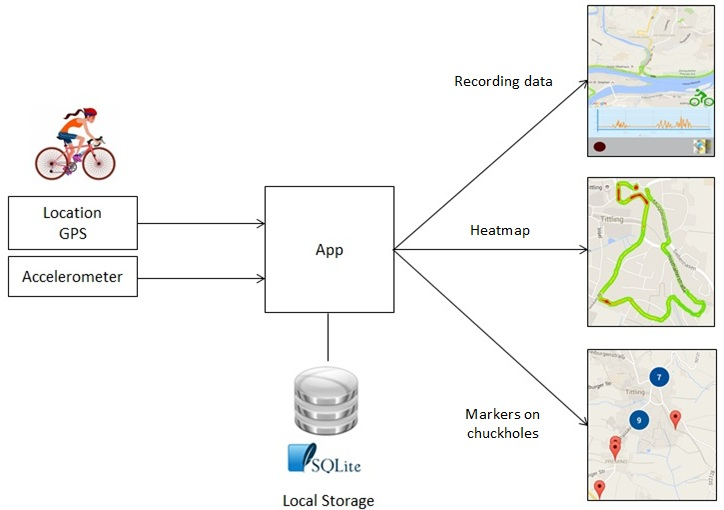
\includegraphics[width=15cm, height=11.5cm]{pic1}
    \end{figure}
    
    
    
    
    \section{App components and features}
	% pictures etc. here
    
    \textbf{Google Map}
    
    All features require a google map. We added it to our app using the Google Maps Android API which automatically handles access to Google Maps servers, data downloading, map display, and response to map gestures. 
    We also used API calls to add heatmap and markers overlay in clusters.
    \textbf{Onboarding}
    
    New users will start with an initiation to get an overview about the mode of operation and main functionalities of the app. In subsequent uses, this phase will be skipped.
    
    
    
    \begin{figure}[H]
    \centering
    \minipage{0.32\textwidth}
    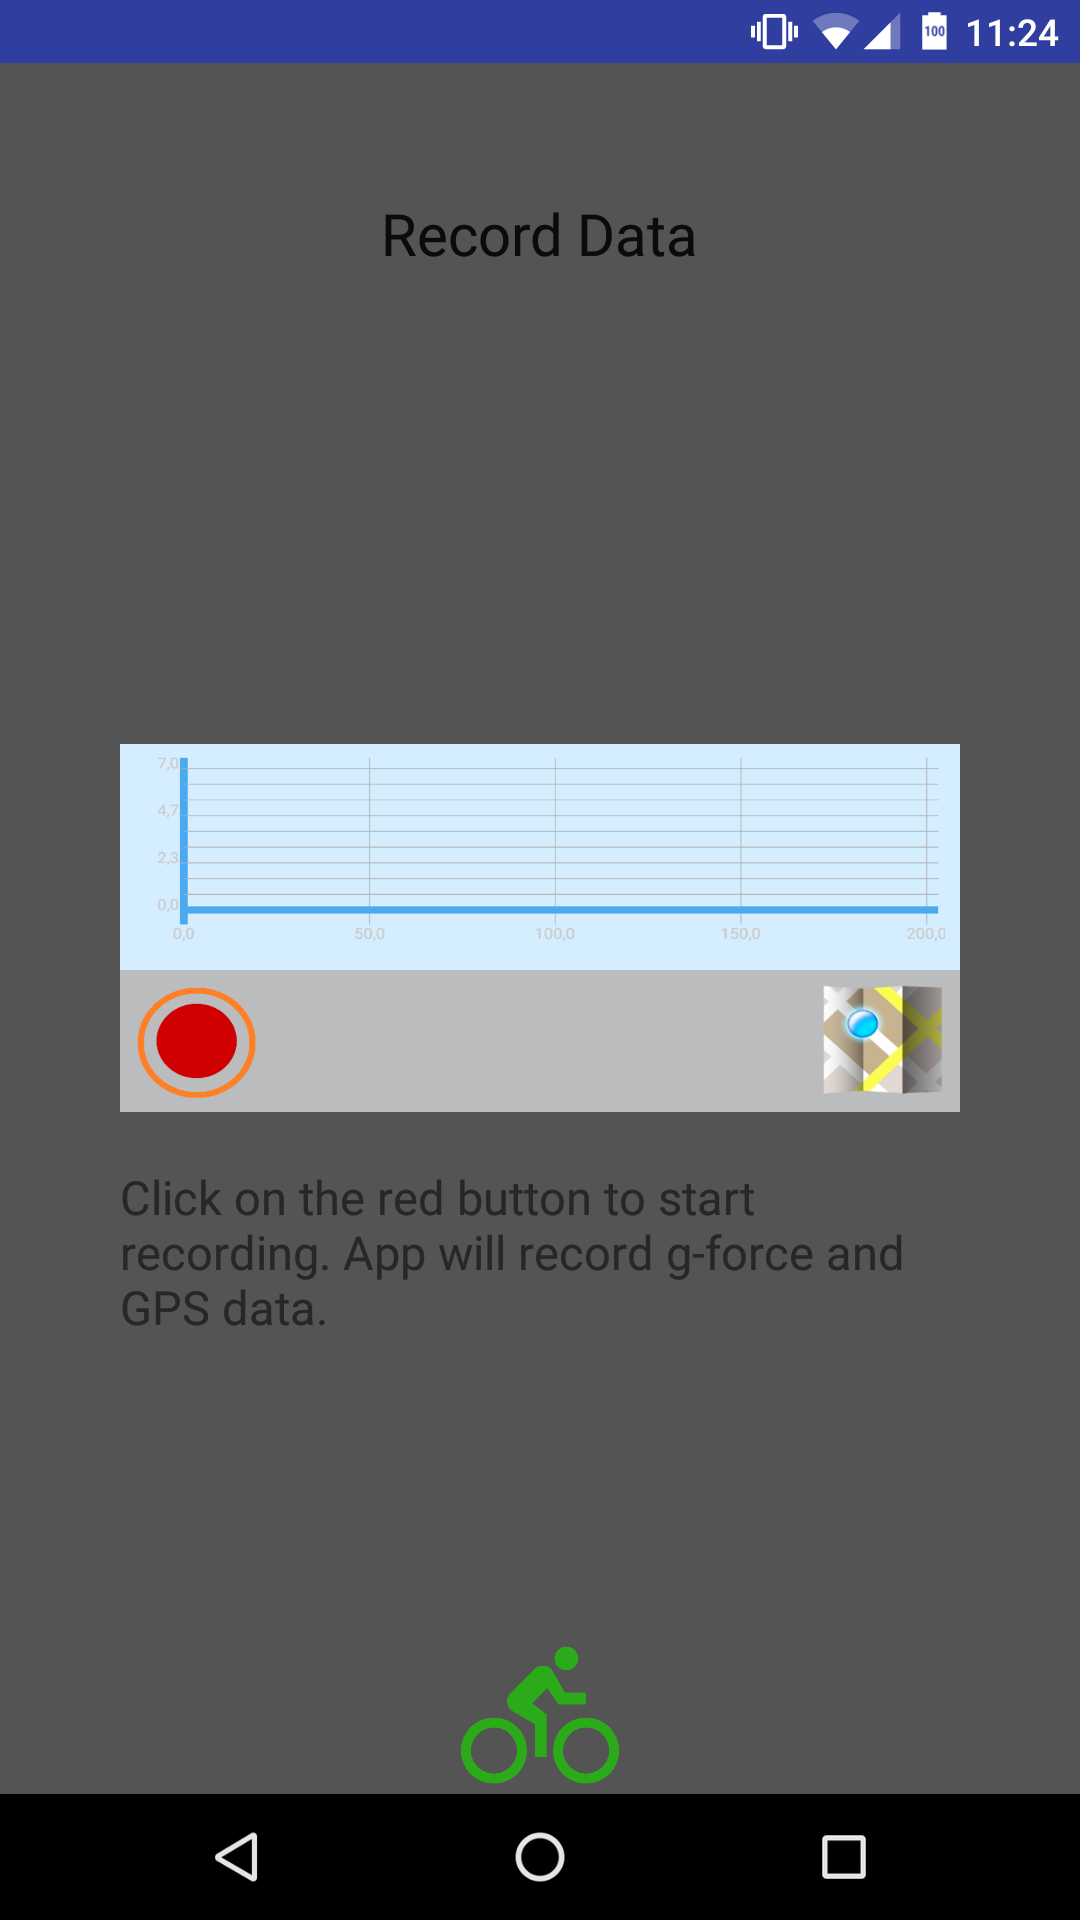
\includegraphics[width=5cm, height=8cm]{pic7} 
    \endminipage\hfill
    \minipage{0.32\textwidth}
    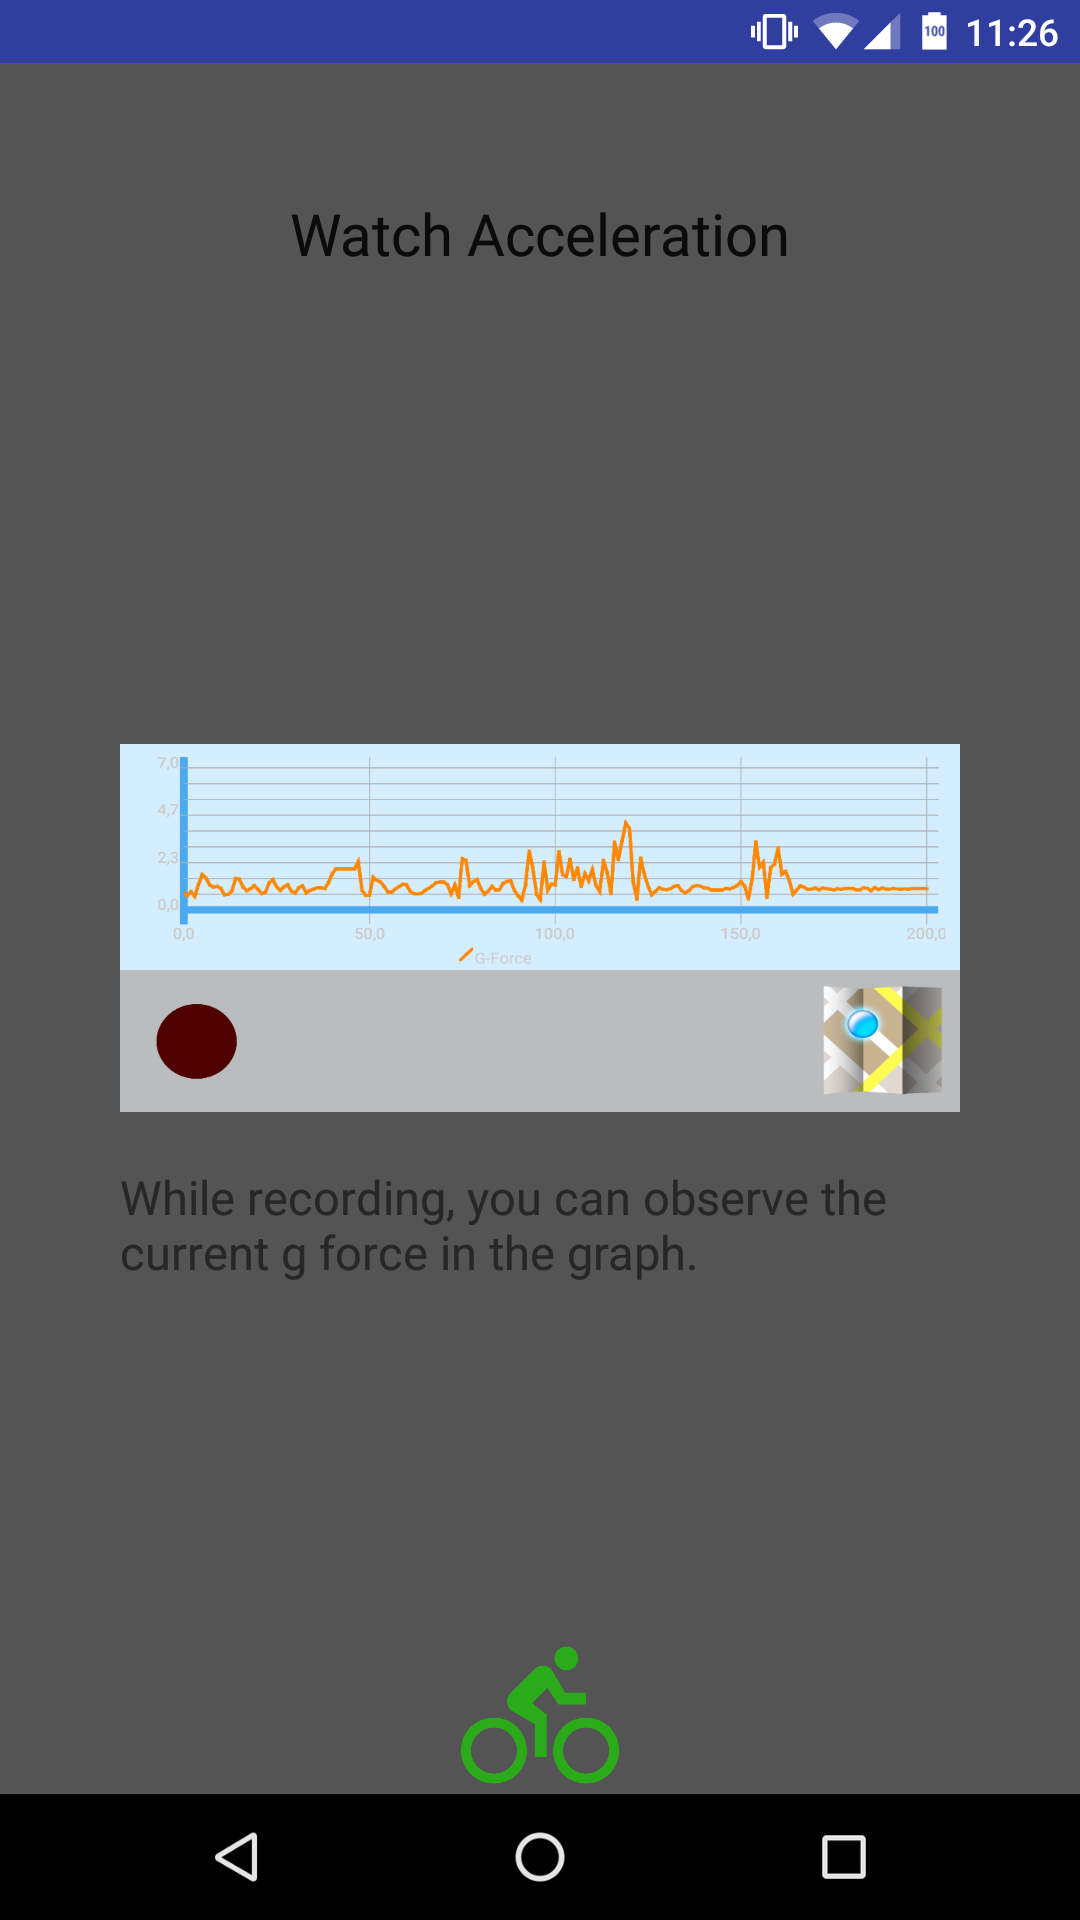
\includegraphics[width=5cm, height=8cm]{pic8}
    \endminipage\hfill
    \minipage{0.32\textwidth}
    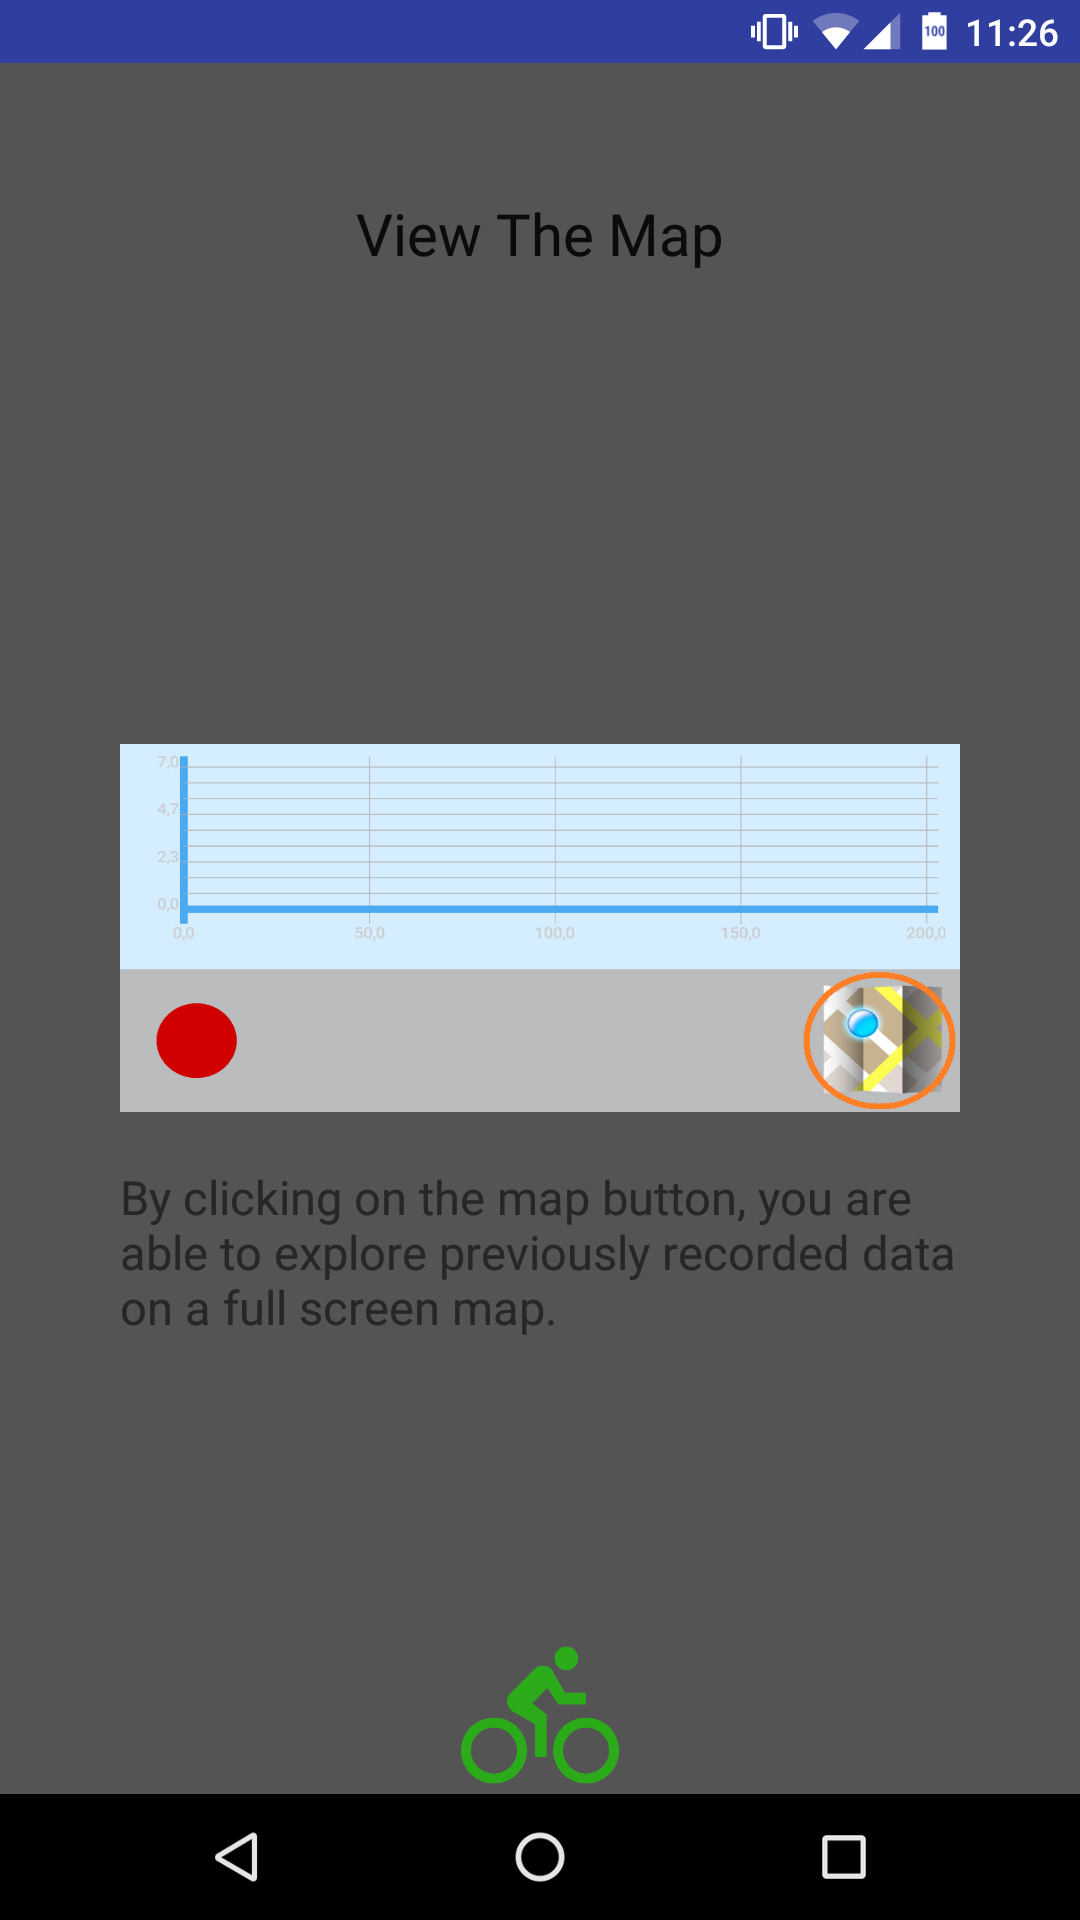
\includegraphics[width=5cm, height=8cm]{pic9}
    \endminipage\hfill
    
    
    
    \end{figure}
    
    
    
    \subsection{ Recording data}
    This feature allows an app user to check the quality of roads during a bike ride.
    
    Using the accelerometer sensor, the app will get the three acceleration axes' values that are necessary to calculate the g-force (force of acceleration) by applying the following formula:
    
   \begin{figure}[H]
	\centering
    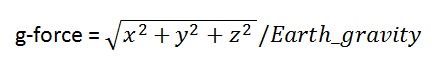
\includegraphics[width=8cm, height=1.5cm]{formule}
    \end{figure}
    
    
    The GPS will provide precise locations of the phone along the ride.
    
    
    
    
    \begin{figure}[H]
	\centering
    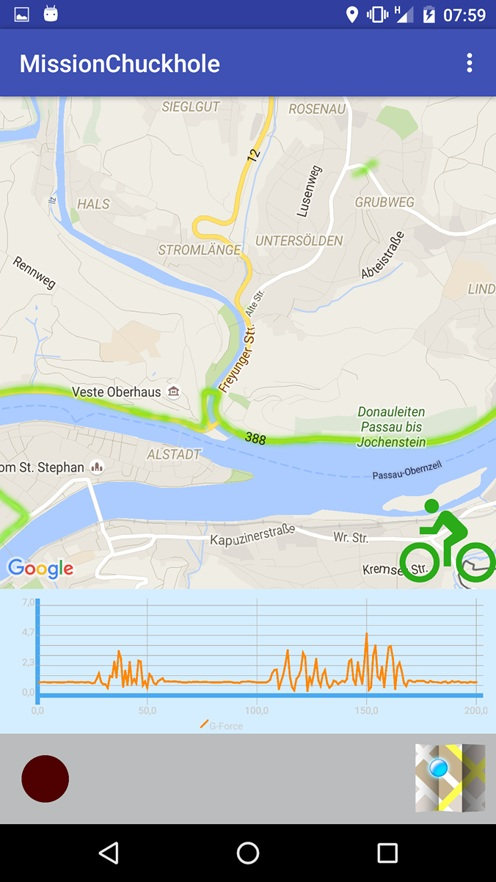
\includegraphics[width=5cm, height=8cm]{pic2}
    \end{figure}
    
    \textbf{Input}
    
    A user has to press the recording button to start the recording phase and once again to stop it.
    For a better visual distinction at the user side, the button has two different colors depending on its status: brown when it is pressed and red otherwise.
    
    A user may also want to use the "Heatmap overlay" or "markers on chuckholes" features and this is possible by pressing the button on the right bottom.
    
    \textbf{Ouput}
    
    The green bike picture is a sign that the ride has just started.
    
    The graph shows the change of the g-force value during the ride and serves as a second output feedback to assure the user that recording is working well.
    
    Both will appear after pressing the recording button.
    
    The third output element is the heatmap that shows the heatmap overlay of previous recording sessions. Moreover, it's dynamically updated to provide real time overlay of the current session.
    
    
    \textbf{Storage}
    
    We opted for a local storage via SQLite database because ...
    
    DataStore is an intermediate data structure between the app features and the SQLite database. Each record of the Datastore contains the following attributes: ...
    
    
    
    
    
    
    
    \subsection{ Heatmap Overlay}
    
    Heatmaps make it easy for viewers to understand the distribution and relative intensity of data points on a google map and was overlaid using the Google Maps Android Heatmap Utility.
    
    We opted for a dynamic heatmapping that requires a collection of 'weighted' latitude/longitude coordinates, each with an intensity value that will determine its associated color.
    Highest values of intensity will be mapped by default to red while lowest ones to green. Concerning the values in between, the given color is generated using interpolation between red and green. 
    
    Our collection will retrieve locations from the DataStore structure and their corresponding g-force values which will represent the intensity parameter. Consequently, locations on a smooth road will get green color while chuckholes will be colored in red and points with average g-forces values will be in yellow.
    
    So an app user will be able to avoid damaged sections of roads or view areas that haven't been checked yet.
     
    \begin{figure}[H]
    \centering
	   
       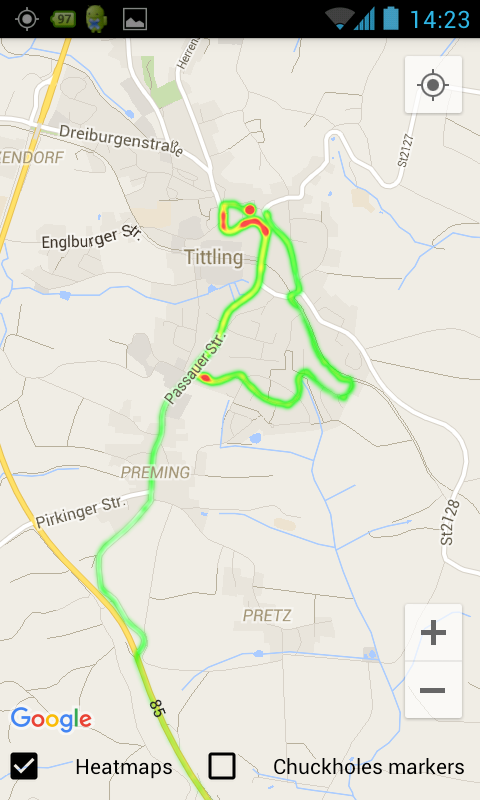
\includegraphics[width=5cm, height=8cm]{pic4}
       
    \end{figure}
    
    Unfortunately, the heatmap utility suffers from some limitations [1]. The main handicap that affects our overlay is that the heatmaps circles overlap at low zoom levels which causes fake coloring and this is due to the fact that the 'Intensity' parameter is additive: the overlap area of two circles of intensity 1 will lead to an overall intensity 2.
    
    \begin{figure}[H]
    \centering
	
	  
	   
       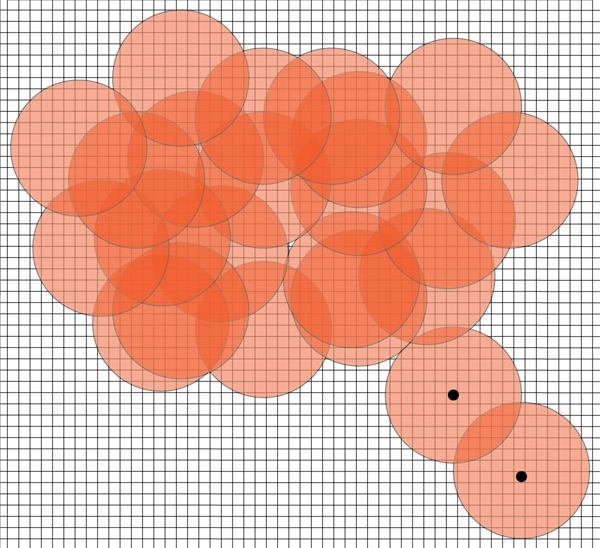
\includegraphics[width=10cm, height=10cm]{pic6}
    
       
    \end{figure}
    
    To overcome this issue, we apply a filtering on our dataset, within a specific zoom range where the overlaps occur, in an attempt to reduce fake coloring of heatmaps.
    
    
    
    \subsection{ Markers on chuckholes Overlay}
    
    This feature is the second output option for an app user who may want to view locations of chuckholes that were detected during a bike ride in a simple way. The locations are retrieved from the DataStore structure described previously. Using the Google Maps Android Marker Clustering Utility, a marker will be overlaid on each location where the corresponding g-force level reaches or exceeds a specific threshold value = 3.5. 
    
    When a user views the map at a high zoom level, individual markers will be shown on the map. When a user zooms out, the markers gather together into clusters, to make viewing the map easier.
    
    \begin{figure}[H]
    \centering
	
	  
	   
       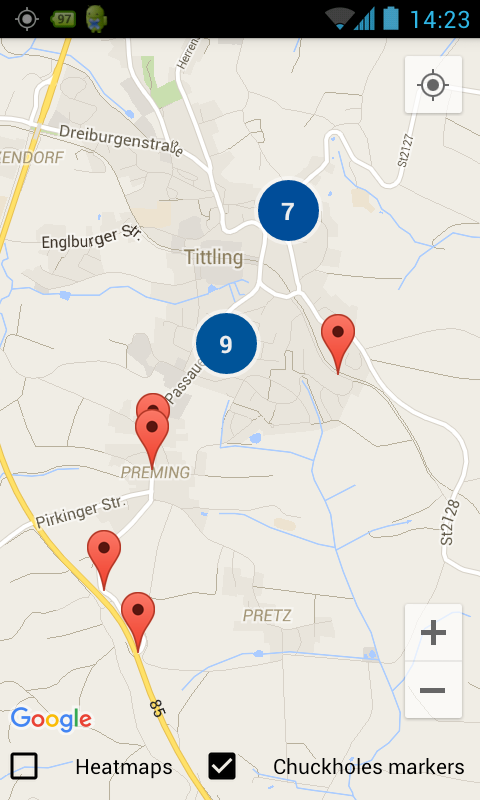
\includegraphics[width=5cm, height=8cm]{pic3}
    
       
        \end{figure}
    
    In case of no chuckhole in the area, the user will get a feedback via a toast message.
    

    
    

    
    
    
    
    
    
    
    
    
    
    
    
    
    
    % bib stuff
    \nocite{*}
    \addtocontents{toc}{\protect\vspace{\beforebibskip}}
    \addcontentsline{toc}{section}{\refname}    
    \bibliographystyle{plain}
    
    \bibliography{./Bibliography}

    
    
    
    
\end{document}
